\documentclass[12pt,a4paper]{article}
\usepackage[utf8]{inputenc}
\usepackage[brazil]{babel}
\usepackage{graphicx}
\usepackage{amssymb, amsfonts, amsmath}
\usepackage{float}
\usepackage{enumerate}
\usepackage[top=2.5cm, bottom=2.5cm, left=1.25cm, right=1.25cm]{geometry}

\begin{document}
\pagestyle{empty}

\begin{center}
  \begin{tabular}{ccc}
    \begin{tabular}{c}
      
\includegraphics[scale=0.25]{../../biblioteca/imagem/brasao-de-armas-brasil} \\
    \end{tabular} & 
    \begin{tabular}{c}
      Ministério da Educação \\
      Universidade Federal dos Vales do Jequitinhonha e Mucuri \\
      Faculdade de Ciências Sociais, Aplicadas e Exatas - FACSAE \\
      Departamento de Ciências Exatas - DCEX \\
      Disciplina: Introdução à Ciência da Computação \quad Semestre: 2022/1\\
      Prof. Dr. Luiz C. M. de Aquino\\
    \end{tabular} &
    \begin{tabular}{c}
      
\includegraphics[scale=0.25]{../../biblioteca/imagem/logo-ufvjm} \\
    \end{tabular}
  \end{tabular}
\end{center}

\begin{center}
  \textbf{Trabalho}
\end{center}

\begin{enumerate}
  \item Considere o problema do circuito hidráulico mostrado na Figura~\ref{fig:tub}. Este sistema está alimentado por um reservatório 
cuja a pressão é mantida constante e igual a $P_r = 10$. As saídas das tubulações desembocam na atmosfera, onde a pressão é 
considerada nula (isto é, $P_a = 0$). Deste modo, a vazão $Q_i$ da $i$-ésima tubulação depende da diferença de pressão $\Delta P_i$ 
de tal modo que $$Q_i = K_iL_i\Delta P_i,$$ onde $K_i$ é a resistência hidráulica e $L_i$ o comprimento da tubulação. Por exemplo, para a 
tubulação $8$ temos que $Q_8 = K_8L_8\Delta P_8$, sendo que $\Delta P_8 = P_1 - P_4$ (ou seja, a pressão que ``entra'' na tubulação pela 
bifurcação $1$ menos a pressão que ``sai'' da tubulação pela bifurcação $4$). Por outro lado, sabe-se que em cada bifurcação a soma das vazões 
deve ser nula. Por exemplo, na bifurcação $4$ temos que $Q_8 - Q_6 - Q_7 = 0$ (aqui note que a vazão que ``entra'' na bifurcação é considerada positiva, 
enquanto que a que ``sai'' é considerada negativa). Considerando essas informações e os dados da Tabela~\ref{tab:dados}, escreva um algoritmo em Python para resolver o sistema de equações lineares de modo a determinar 
as vazões em cada tubulação e as pressões em cada bifurcação.

\begin{figure}[!htb]
 \centering
 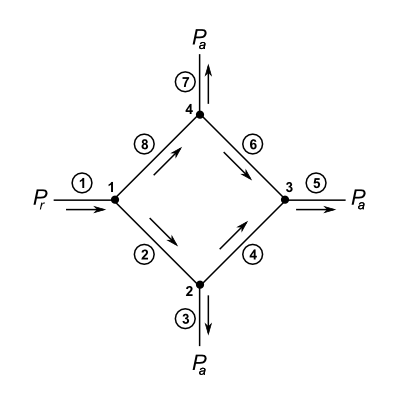
\includegraphics[scale=0.75]{imagem/tubulacao.png}
 \caption{Esquema do circuito hidráulico.}
 \label{fig:tub}
\end{figure}

\begin{table}[!htb]
 \centering
 \begin{tabular}{c|c|c}
  Tubulação $i$ & $K_i$ & $L_i$ \\ \hline
  1 & 0,02 & 1,0 \\ \hline
  2 & 0,005 & 2,0 \\ \hline
  3 & 0,085 & 0,5 \\ \hline
  4 & 0,02 & 1,0 \\ \hline
  5 & 0,075 & 0,5 \\ \hline
  6 & 0,085 & 0,5 \\ \hline
  7 & 0,015 & 2,0 \\ \hline
  8 & 0,01 & 1,0 
 \end{tabular}
 \caption{Resistência hidráulica e comprimento das tubulações.}
 \label{tab:dados}
\end{table}

\end{enumerate}

\end{document}